\chapter{La rupture en mécanique}\label{Ch-rupt}
La mécanique de la rupture s'intéresse à la formation et à la propagation de fissures
macroscopiques dans les structures, ce qui peut conduire à la séparation d'un corps en deux
parties disjointes suite à une phase d'amorçage qui a vu le développement de microcavités,
microfissures... mais les fissures peuvent aussi s'arrêter.
Le mode de rupture peut être fragile (sans déformation plastique) ou ductile (avec déformation
plastique).

\medskip
La \textcolorblue{résilience} est le rapport de l'énergie nécessaire pour rompre une pièce sur la
section droite de matière rompue: elle caractérise l'énergie nécessaire pour produire la rupture.
La résilience évolue avec la température (la température de transition caractérise le passage
d'une mode de rupture à un autre : fragile ou ductile). Par ailleurs, le mode de rupture dépend de l'état de contrainte, en particulier de la \emph{triaxialité des contraintes} (rapport du premier sur le second invariant, voir paragraphe \ref{Sec-TensS}): un matériau très plastique peut développer des ruptures fragiles; un matériau sans plasticité ne présentera que des ruptures fragiles.

\medskip
En fonction du chargement et du matériau considéré:
\begin{itemize}
   \item si le milieu est globalement plastique ou viscoplastique, on recourra à la mécanique
	non linéaire de la rupture, ou approche locale (description fine des contraintes et déformations
	en pointe de fissure à l'aide de modèles non linéaires);
   \item si la plasticité absente ou très confinée, on utilisera la mécanique linéaire de la rupture.
\end{itemize}

%\medskip
%1920 : Griffith montre que la rupture d'un milieu élastique fragile peut être caractérisé par
%une variable que l'on appellera plus tard le taux de restitution d'énergie.
%
%1956 : Irwin étudiant les singularités du champ de contraintes introduit la notion de facteur
%d'intensité des contraintes.
%
%Puis essors des développements numériques et traitement des problèmes non linéaires.





\medskip
\section{Approches globale et locale}
On distingue deux approches :
\begin{itemize}
   \item \textcolorblue{Approche globale}: le principal avantage est la relative simplicité d'application
	aux calculs éléments finis ou analytiques grace à des \emph{grandeurs scalaires représentant l'état de
	la fissure}, mais qui sont des approximations qui peuvent \textcolorred{manquer de pertinence};
   \item \textcolorblue{Approche locale}: qui veut \emph{modéliser finement le comportement réel},
	mais se confronte à la \textcolorred{singularité des contraintes en fond de fissure}.
\end{itemize}
%%%%%%%%%%%%%%%%%%%%
\medskipvm
D'un point de vue numérique, les deux approches nécessitent des maillages fins en pointe de
fissure afin de décrire le front de fissure et de permettre le calcul de la concentration des contraintes
et déformations.
Il faut ajouter également des modèles de comportement adaptés:
\begin{itemize}
   \item l'approche globale nécessite un \textcolorblue{maillage rayonnant} avec faces perpendiculaires
	au front de fissure;
   \item alors que l'approche locale impose un \textcolorblue{maillage fin} (calcul des contraintes), dont la
	taille est imposée ainsi que le type d'éléments.
\end{itemize}
%%%%%%%%%%%%%%%%%%%%
\medskipvm
Les fissures sont souvent trop complexes pour être parfaitement reproduites, ce qui impose
des approximations du domaine, ce qui rend le choix du type d'éléments et leur taille encore
plus critique.

La modélisation du comportement des matériaux est importante puisque directement
liée au calcul des sollicitations en pointes de fissure, qui de plus apparaissent toujours dans
des zones où les sollicitations sont complexes (fatigue, fluage, plasticité, endommagement...).

La \emph{modélisation de l'avancée de la fissure} conduit à de très fortes non linéarités
(avec des problèmes de convergence dans les algorithmes).
De plus, la modélisation de l'avancée de fissure est liée à la discrétisation faite, donc est
liée à la taille des éléments.

Les mailleurs automatiques sont souvent incapables de mener à bien leur tâche car
il y a une incompatibilité entre les dimensions de la structure et la finesse nécessaire
pour la fissure, et parce que les approches locale et globale ont des spécificités de maillage
différentes et difficiles à prendre en compte.
Il est donc souvent nécessaire de développer ses propres outils de maillage.
De plus beaucoup de critères mis au point en 2D ne sont pas forcément valables
en 3D.

\medskip
Les problèmes actuels sur lesquels portent la recherche sont:
\begin{itemize}
   \item la \emph{propagation}, qui reste un domaine numérique difficile à aborder, en
	particulier les \emph{critères de propagation} de fissure, surtout en 3D et/ou en dynamique.
   \item les \emph{mailleurs} (voir ci-dessus), et même en amont, les \emph{critères de maillage},
	surtout en 3D.	
\end{itemize}
%%%%%%%%%%%%%%%%%%%%%%%
\medskipvm
On opte également pour une approche couplée essais / calculs:
\begin{itemize}
   \item développement des paramètres pertinents en mécanique de la rupture;
   \item développement d'outils analytiques et critères associés;
   \item développement / validation des critères.
\end{itemize}

\medskip
\paragraph{Approches numériques des fissures}
\begin{description}
   \item[\textcolorblue{Fissure droite} sollicitée en mode I]
	Le trajet de propagation peut être connu \emph{a priori}, et on trouve les
	méthodes de déboutonnage dans lesquelles la moitié de la structure est
	maillée et les nœuds situés sur la ligne de propagation sont libérés
	à mesure que la fissure avance. \textcolorred{Mais} il faut relâcher les nœuds
	progressivement en appliquant des forces nodales physiquement
	pertinentes.
   \item[\textcolorblue{Fissure courbe}]\mbox{}
\begin{itemize}
\item méthodes de remaillage :
	voir problème de maillage
   \item éléments d'interface :
	le trajet de la fissure est imposé par la discrétisation et il faut choisir
	la loi de décohésion à l'interface.
	\end{itemize}
   \item[\textcolorblue{Élément avec un nœud supplémentaire}]
	au quart de ses côtés (ou ayant son nœud intermédiaire déplacé), qui
	permet d'intégrer exactement la singularité élastique, mais il reste
	nécessaire de disposer d'un outil spécifique de remaillage.
   \item[Méthodes \textcolorblue{sans maillage}] Elles permettent de s'affranchir
	des problèmes liés à la connaissance trop intime de la fissure;
   \item[Méthodes utilisant la \textcolorblue{partition de l'unité}]
	Elles permettent de s'affranchir du maillage explicite de la fissure dont la
	description se fait au moyen d'éléments géométriques ou de fonctions
	de niveau pour le problème 3D.
\end{description}
Notons que les méthodes de remaillage peuvent introduire des singularité dans la
discrétisation temporelle qui sont peu souvent mentionnées.



\medskip
\section{Mécanique linéaire de la rupture}

\medskip
\subsection{Concentrations de contraintes des défauts}
%\colormagenta\textbf{Un peu d'histoire:}
\begin{histoire}%
On a souvent attribué aux défauts du matériau la cause principale de la rupture fragile.
Sur la base d'une analyse des contraintes, Kirsch (1898)\index[aut]{Kirsch} et
Inglis\index[aut]{Inglis (Charles), 1875-1952, Anglais} (1913, cité au 8ème symposium  de mécanique des roches en 1966)
avaient déjà donné des solutions analytiques pour le calcul du facteur de concentration des
contraintes pour des plaques infinies soumises à la traction avec respectivement un trou circulaire
et un trou elliptique.

\medskip
Mais le facteur de concentration des contraintes devenait infini dans le cas d'une fissure et cela signifiait
que des contraintes externes très faibles suffisaient pour la rupture d'un solide fissuré, ce qui est en
contradiction avec la réalité.
\end{histoire}
\colorblack

\medskip
Inglis,\index[aut]{Inglis (Charles), 1875-1952, Anglais} donc, en 1913, a montré l'effet de \textcolorblue{concentration de contraintes}.
%%%%%%%%%%%%%%%%%%%%%%%%%
\medskipvm
Considérons une plaque avec un trou elliptique, de grand axe $2a$ et petit axe $2b$, dont la largeur $\ell$ est très supérieure aux dimensions du trou (i.e. $\ell\gg 2a$) et soumise à une contrainte nominale constante
$\sigma$ --- voir figure~\ref{fig:fissure}.
La contrainte en pointe de fissure (point A) est:
\begin{equation} \sigma_A = \sigma \left( 1+\frac{2a}b\right) \end{equation}
Le \textcolorblue{facteur de concentration de contraintes $k_f$} est défini comme $k_f = \sigma_A/\sigma$:
\begin{itemize}
   \item si $a=b$, alors $k_f=3$;
   \item si $a\rightarrow\infty$, Inglis\index[aut]{Inglis (Charles), 1875-1952, Anglais} propose $\sigma_A=\sigma (1+2\sqrt{a/\rho})$,
	où $\rho=b^2/A$ est le rayon en pointe de fissure;
   \item si $a\gg b$, alors $\sigma_A=2\sigma \sqrt{\frac{a}{\rho}}$.
\end{itemize}
\begin{figure}[ht]\centering
\subfloat[titre ?]{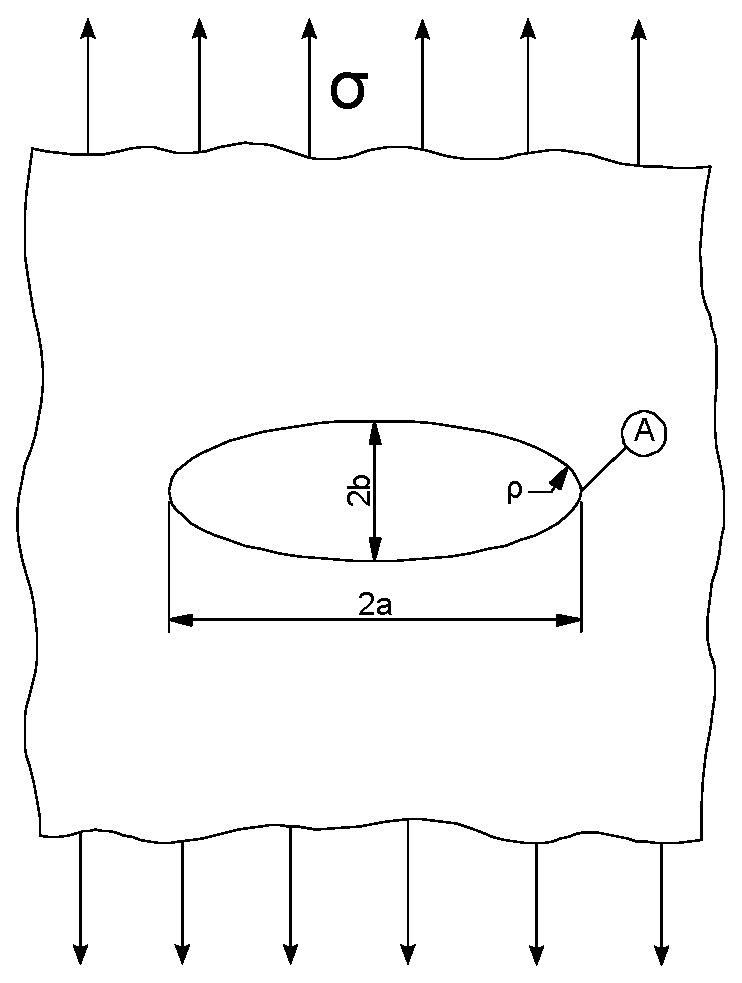
\includegraphics[height=45mm]{fissure.eps}\label{fig:fissure}}\qquad\qquad
\subfloat[titre ?]{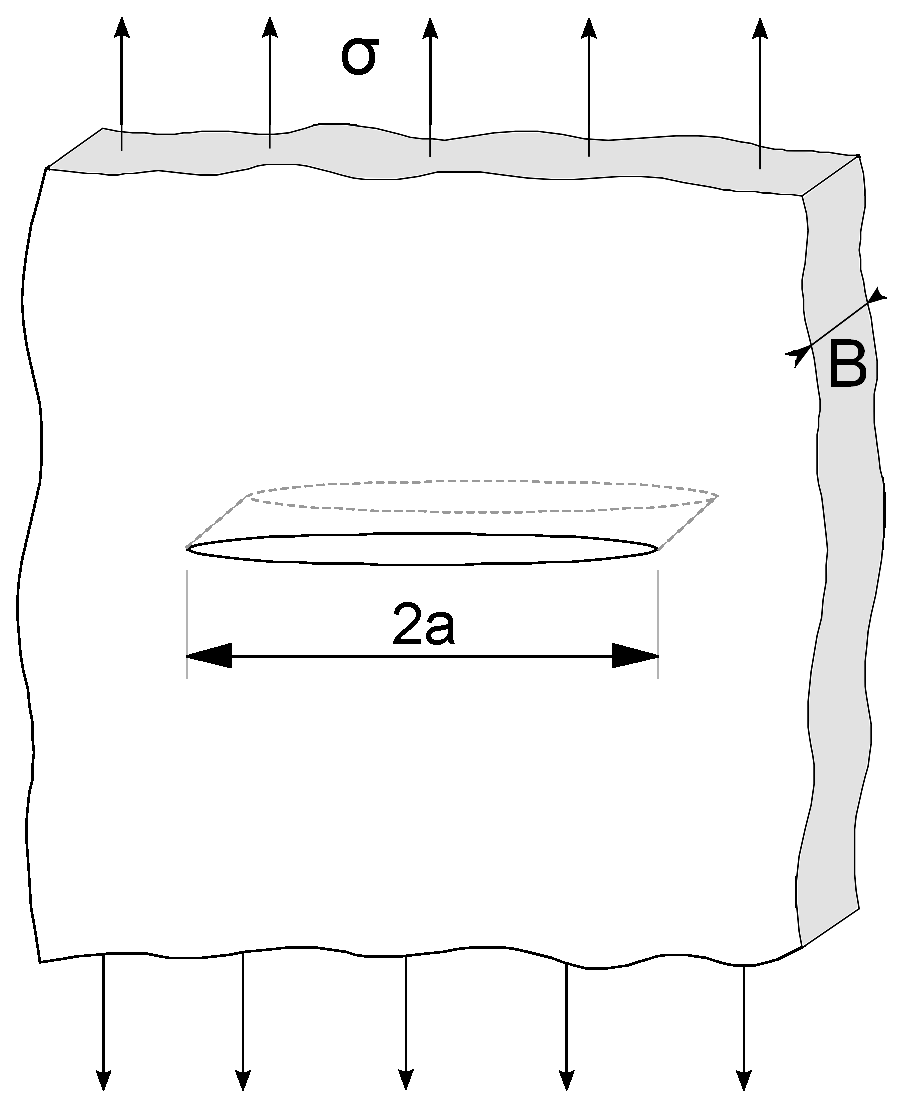
\includegraphics[height=45mm]{fissure2.eps}\label{fig:fissure2}}
\caption{Titre ?}
\end{figure}
\subsection{Équilibre énergétique}
\begin{histoire}%
La mécanique de la rupture a été inventée pendant la Première Guerre mondiale par
l'ingénieur aéronautique anglais A. A. Griffith\index[aut]{Griffith (Alan Arnold), 1893-1963, Anglais}
pour expliquer la rupture des matériaux fragiles.
%%%%%%%%%%%%%%%%%%%%
\medskipvm
Le travail de Griffith\index[aut]{Griffith (Alan Arnold), 1893-1963, Anglais} a été motivé par deux
faits contradictoires:
\begin{enumerate}
\item La contrainte nécessaire pour rompre un verre courant est d'environ 100~MPa;
\item La contrainte théorique nécessaire à la rupture de liaisons atomiques est d'environ 10\,000~MPa.
\end{enumerate}
\sbox{\MaBoiteAvecPhotos}{\setlength{\tabcolsep}{0pt}\scriptsize%
\begin{tabular}{c}%
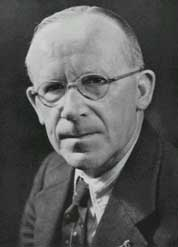
\includegraphics[height=\the\HauteurDesPhotos]{Griffith}\\%
Griffith%
\end{tabular}}
\medskip
\ImageADroite{%
Une théorie était nécessaire pour concilier ces observations contradictoires.
En outre, les expérimentations sur les fibres de verre que Griffith\index[aut]{Griffith (Alan Arnold), 1893-1963, Anglais}
lui-même a mené suggèrent que la contrainte de rupture augmente d'autant plus que le diamètre
des fibres est petit.
Par conséquent il en déduit que le paramètre de résistance uniaxiale à la rupture $R_r$,
utilisé jusqu'alors pour prédire les modes de défaillance dans le calcul des structures, ne pourrait pas
être une valeur indépendante des propriétés du matériau.\\
\indent
Griffith\index[aut]{Griffith (Alan Arnold), 1893-1963, Anglais} suggère que la faiblesse de la résistance
à la rupture observée dans ses expériences, ainsi que la dépendance de l'intensité de cette résistance,
étaient due à la présence de défauts microscopiques préexistant dans le matériau courant.
}

\medskip
Pour vérifier l'hypothèse de défauts préexistants, Griffith\index[aut]{Griffith (Alan Arnold), 1893-1963, Anglais}
a introduit une discontinuité artificielle dans ses échantillons expérimentaux.
La discontinuité artificielle était une forme de fissure débouchante plus importante que les autres
discontinuités supposées préexistantes dans l'échantillon.

\medskip
Les expériences ont montré que le produit de la racine carrée de la longueur de défauts et la
contrainte à la rupture étaient à peu près constante.
\end{histoire}
\colorblack

\medskip
En 1920, Griffith\index[aut]{Griffith (Alan Arnold), 1893-1963, Anglais} considère le cas d'une plaque
d'épaisseur $B$ contenant une fissure de longueur $2a$ et dont la largeur $\ell$ est très supérieure
aux dimensions de la fissure (i.e. $\ell\gg 2a$) et à son épaisseur (i.e. $\ell\gg B$), soumise à une contrainte nominale constante $\sigma$ --- voir figure~\ref{fig:fissure2}.
%%%%%%%%%%%%%%%%%%%%
\medskipvm
Sous l'hypothèse de contrainte plane, Griffith\index[aut]{Griffith (Alan Arnold), 1893-1963, Anglais} montre
que l'équilibre énergétique est:
\begin{equation} \frac{\dd E}{\dd A} = \dfrac{\dd\Pi}{\dd A}+\frac{\dd W_s}{\dd A} = 0 \end{equation}
où $A=2aB$ est l'aire de la fissure, $\dd A$ l'accroissement de fissure, $E$ l'énergie
totale, $\Pi$ l'énergie potentielle et $W_s$ l'énergie nécessaire pour la progression du
défaut.

\medskip
Griffith\index[aut]{Griffith (Alan Arnold), 1893-1963, Anglais} montre également que l'énergie potentielle
$\Pi$ est reliée à l'énergie potentielle de la plaque sans défaut par la relation:
\begin{equation} \Pi=\Pi_0 -\left( \dfrac{\pi a \sigma^2}{E} \right) 2aB \end{equation}
et que $W_s$ est donnée par:
\begin{equation} W_s=4aV\gamma_S\end{equation}
avec $\gamma_s$ l'énergie de progression du défaut par unité de surface.
L'équation d'équilibre énergétique de Griffith\index[aut]{Griffith (Alan Arnold), 1893-1963, Anglais} conduit à:
\begin{equation}-\frac{\dd\Pi}{\dd A}=\frac{\dd W_s}{\dd A}\end{equation} et donc:
\begin{equation}\frac{\pi a\sigma^2}{E}=2\gamma_s\end{equation}
%%%%%%%%%%%%%%%%%%%%
\medskipvm
Griffith\index[aut]{Griffith (Alan Arnold), 1893-1963, Anglais} obtient donc la \textcolorblue{contrainte
globale de rupture $\sigma_f$} pour les matériaux fragiles (uniquement):
\begin{equation} \sigma_f = \sqrt{\dfrac{2E\gamma_s}{\pi a}} \end{equation}
Ces travaux seront complétés par Irwin\index[aut]{Irwin (George Rankine), 1907-1998, Américain} afin de
prendre en compte le cas de la rupture ductile (pour les matériaux métalliques).
Ce dernier obtient la contrainte globale de rupture:
\begin{equation} \sigma_f = \sqrt{\dfrac{2E(\gamma_s+\gamma_p)}{\pi a}} \end{equation}
où $\gamma_p$ est l'énergie plastique de progression de fissure par unité de surface
\textcolorgreen{(i.e. en rupture fragile $W_f=\gamma_s$, et en rupture ductile $W_f=\gamma_s+\gamma_p$)}.


\medskip
\subsection{Taux d'énergie libre $G$}\index{Taux de restitution d'énergie $G$}

\medskip
\begin{histoire}%
L'œuvre de Griffith\index[aut]{Griffith (Alan Arnold), 1893-1963, Anglais} a été largement ignorée par
la communauté des ingénieurs jusqu'au début des années 1950.
Les raisons semblent être que, pour les matériaux employés dans la réalisation des structures,
le niveau réel d'énergie nécessaire pour causer la rupture est de plusieurs ordres de grandeur
supérieur à l'énergie de surface correspondante et que, dans les matériaux de construction il
y a toujours des déformations élastiques en fond de fissure ce qui rend l'hypothèse du milieu
élastique linéaire avec contraintes infinie en pointe de la fissure tout à fait irréaliste.

\medskip
La théorie de Griffith\index[aut]{Griffith (Alan Arnold), 1893-1963, Anglais} concorde parfaitement avec
les données expérimentales sur des matériaux fragiles tels que le verre. Pour des matériaux ductiles
tels que l'acier, l'énergie de surface prédite par la théorie de Griffith\index[aut]{Griffith (Alan Arnold), 1893-1963, Anglais}
est souvent irréaliste.
Un groupe de travail dirigé par G. R. Irwin\index[aut]{Irwin (George Rankine), 1907-1998, Américain} à
l'US Naval Research Laboratory, constitué durant la  Seconde Guerre mondiale, a réalisé que la plasticité
doit jouer un rôle important dans la rupture  des matériaux ductiles.

\medskip
Dans les matériaux ductiles (et même dans des matériaux qui semblent être fragiles), une zone
plastique se développe en front de fissure.
L'augmentation de la dimension de la zone plastique est fonction de l'augmentation de la charge jusqu'à
ce que la fissure se propage libérant les contraintes en arrière du fond de fissure.
Le cycle de chargement/libération de chargement plastique aux abords du front de fissure conduit à
la dissipation d'énergie comme le ferait un traitement thermique de relaxation de contrainte.
Par conséquent, un terme dissipatif doit être ajouté à la relation de l'équilibre énergétique tel
qu'élaborée par Griffith pour les matériaux cassants.
En termes physiques, de l'énergie supplémentaire est nécessaire pour que la propagation des fissures
se produise dans les matériaux ductiles si on les compare aux matériaux fragiles.
%%%%%%%%%%%%%%%%%%%%
\medskipvm
La stratégie d'Irwin\index[aut]{Irwin (George Rankine), 1907-1998, Américain} a été de partitionner
l'énergie en:
\begin{enumerate}
\item énergie stockée en déformation élastique (effet ressort) qui se libère lors de la propagation
d'une fissure et;
\item énergie dissipée qui comprend la dissipation plastique et l'énergie de surface (et toutes les autres
forces dissipatives qui peuvent être au travail).
\end{enumerate}
\end{histoire}
\colorblack

\medskip
Poursuivant ses travaux, Irwin\index[aut]{Irwin (George Rankine), 1907-1998, Américain} propose en 1957
une mesure énergétique $G$ pour caractériser la rupture:
\begin{equation} G = \dfrac{\dd\Pi}{\dd A} \end{equation}
\textcolorgris{En négligeant l'énergie cinétique, la puissance disponible pour ouvrir une fissure
de surface $A$ est égale à la variation d'énergie potentielle totale, résultat de la variation de l'énergie
élastique stockée dans la structure et de la variation d'énergie liée aux forces extérieures.
Cette contribution mécanique est appelée taux de restitution d'énergie.}

$G$ est la quantité d'énergie permettant un accroissement de fissure de $\dd A$ et est aussi appelé
force d'expansion de fissure ou \textcolorblue{taux de restitution d'énergie}.\index{Taux de restitution d'énergie $G$}

\medskip
En revenant au cas traité par Griffith,\index[aut]{Griffith (Alan Arnold), 1893-1963, Anglais} on obtient
en contraintes planes:
\begin{equation} G = \dfrac{\pi a\sigma^2}{E} \end{equation}
et ainsi, \textcolorblue{une fissure va progresser si $G$ atteint une valeur critique $G_c$}:
\begin{equation} G_c = \dfrac{\dd W_s}{\dd A}=2\gamma_s \end{equation}
où $\gamma_s$ est l'énergie de progression du défaut par unité de surface.
$G_c$ est la mesure de ténacité à la rupture du matériau.


\medskip
\subsection{Facteur d'intensité de contrainte $K$}\index{Facteur d'intensité de contrainte $K$}

\medskip
\begin{histoire}%
Une autre réalisation importante du groupe de travail dirigé par Irwin a été de trouver une méthode
de calcul de la quantité d'énergie disponible pour une fracture au niveau de la contrainte asymptotique
et les champs de déplacement autour d'un front de fissure dans un solide idéalement élastique.

C'est le  facteur d'intensité de contrainte.\index{Facteur d'intensité de contrainte $K$}
\end{histoire}
\colorblack

\begin{figure}[ht]\centering
\subfloat[titre ?]{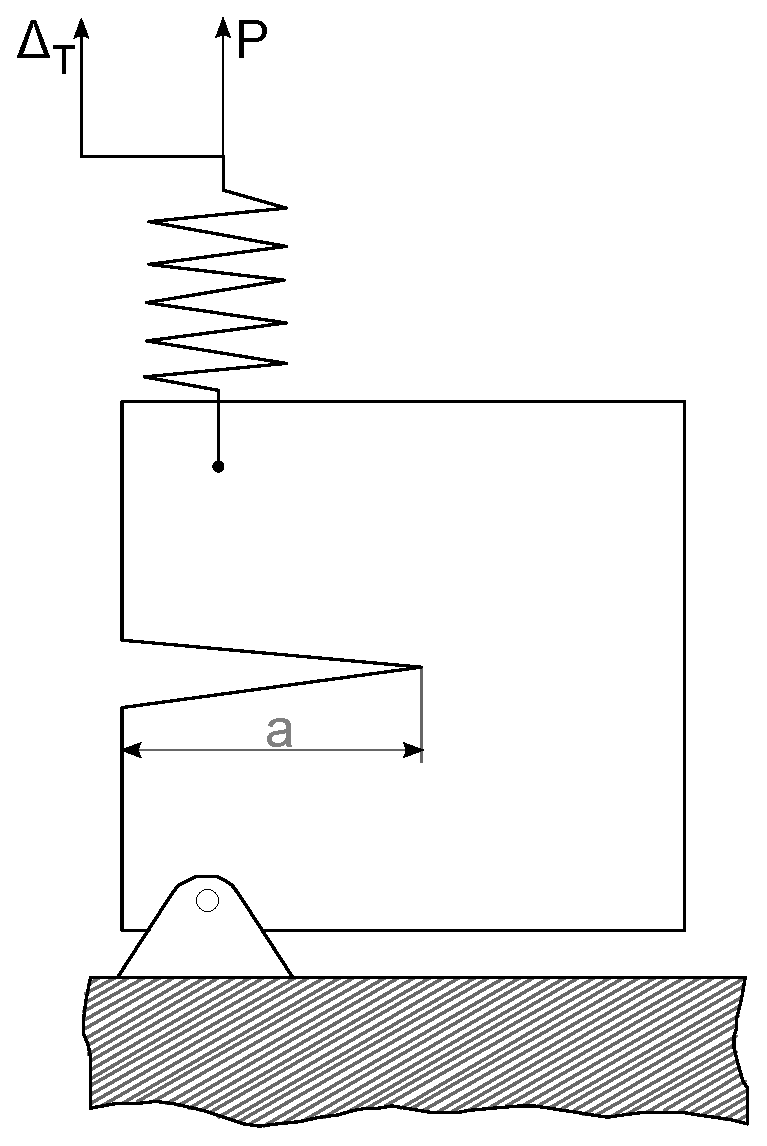
\includegraphics[height=45mm]{fissIrwin.eps}}\qquad\qquad
\subfloat[titre ?]{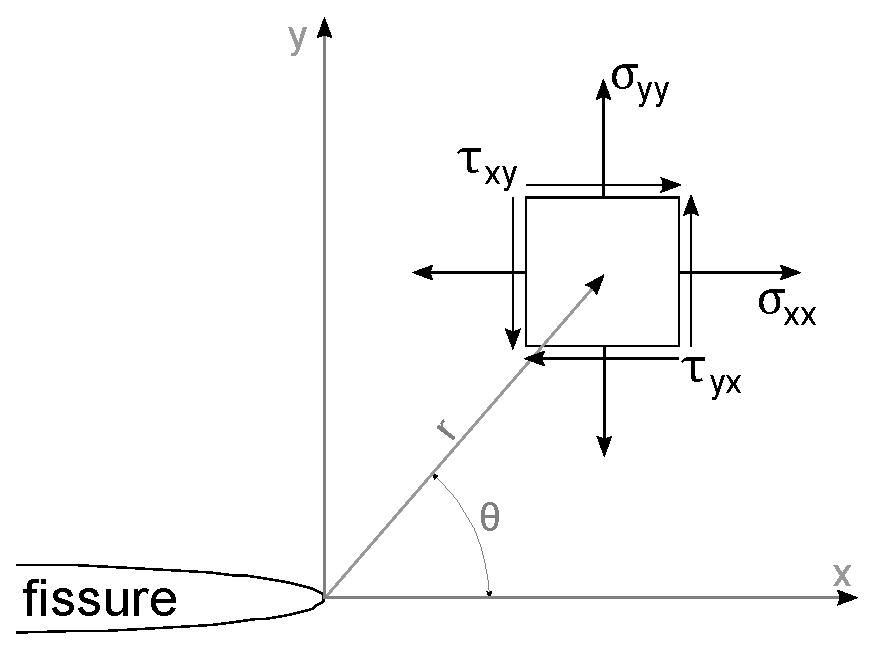
\includegraphics[height=45mm]{fisspol.eps}}
\caption{Titre?}
\end{figure}
Pour certaines configurations de structures soumises à un chargement, on peut démontrer que:
\begin{equation} \sigma_{ij} = \frac{k}{\sqrt{r}} f_{ij}(\theta) + \dsum_{m=0}^\infty A_m r^{m/2} g_{ij}(\theta) \end{equation}
où $f_{ij}(\theta)$ est une fonction adimensionnelle, et $(r, \theta)$ les coordonnées polaires en fond
de fissure.
En posant:
\begin{equation} K = k\sqrt{2\pi} \end{equation}
Irwin\index[aut]{Irwin (George Rankine), 1907-1998, Américain} montre en 1957 qu'au voisinage du fond de
fissure, on a:
\begin{align}
&\lim_{r\rightarrow0} \sigma_{ij}^{(I)} = \frac{K_I}{\sqrt{2\pi r}} f_{ij}^{(I)}(\theta) \\
&\lim_{r\rightarrow0} \sigma_{ij}^{(II)} = \frac{K_II}{\sqrt{2\pi r}} f_{ij}^{(II)}(\theta) \\
&\lim_{r\rightarrow0} \sigma_{ij}^{(III)} = \frac{K_III}{\sqrt{2\pi r}} f_{ij}^{(III)}(\theta)
\end{align}
trois modes de chargements pouvant s'appliquer à une fissure. Ces trois modes sont donnés à la~\fig{Fig-modesR}.
Pour un mode mixte général il vient:
\begin{equation} \sigma_{ij}^{(total)} = \sigma_{ij}^{(I)} + \sigma_{ij}^{(II)} + \sigma_{ij}^{(III)} \end{equation}
\begin{figure}[htb]
\centering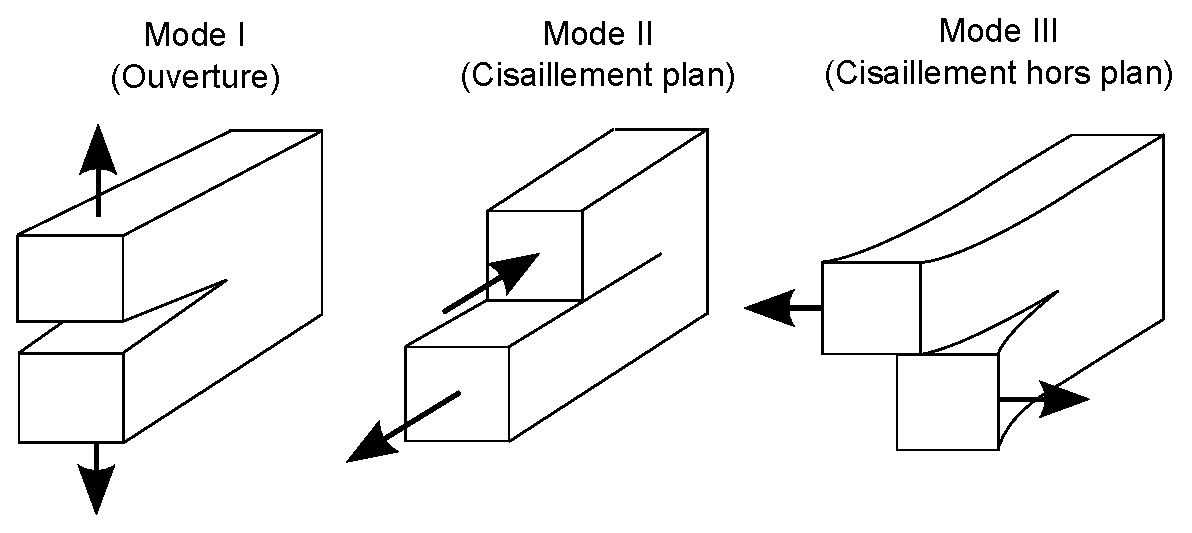
\includegraphics[height=55mm]{modesR.eps}
\caption{Modes de chargement d'une fissure}\label{Fig-modesR}
\end{figure}


\medskip\colorgreen
La détermination de $K$ peut se faire analytiquement uniquement pour des géométries simples.
Pour des cas plus complexes, il faut le faire numériquement ou expérimentalement.
\begin{itemize}
\item Par les contraintes: par exemple $K_I$ sera pris égale à la valeur obtenue (post-traitée)
de $\sigma_{yy}\sqrt{2\pi r}$ en fond de fissure. Cette méthode simple et directe est peu
précise (car on utilise les contraintes).
\item Par les déplacements: $K_I$ est obtenu par $\nu \sqrt{2\pi/r}$ en fond de fissure (obtenu
par extrapolation), $\nu$ étant le coefficient de Poisson.
Cette méthode relativement simple nécessite de raffiner le maillage
autour de la fissure et sa précision n'est pas excellente (environ 5\%).
\end{itemize}
\colorblack

\medskip
\colorgris
ATTENTION : il ne faut pas confondre $K_I$ avec $K_t$ qui est le facteur de concentration
de contrainte, sans dimension, et qui caractérise le rapport entre la contrainte normale
maximale et la contrainte à l'infini au voisinage d'une entaille.
\begin{equation} K_t = \dfrac{\sigma_{22 max}}{\sigma_\infty} \end{equation}
\colorblack

\medskip
Si l'on reprend le cas de la plaque plane semi-infinie traitée par Griffith,\index[aut]{Griffith (Alan Arnold), 1893-1963, Anglais}
en exprimant le champ de contraintes au voisinage du fond de fissure et en faisant tendre $\theta$ vers $0$,
on obtient des relations entre $G$ et $K$:
\begin{align}
&G_I = \dfrac{K_I^2}E \quad \text{et en déformations plane:}\quad
G_I = (1-\nu^2)\dfrac{K_I^2}E \\
&G_{II} = \dfrac{K_{II}^2}E \qquad \text{et en déformations plane:}\quad
G_{II} = (1-\nu^2)\dfrac{K_{II}^2}E \\
&G_{III} = (1+\nu)\dfrac{K_{III}^2}E
\end{align}

\medskip
\subsection{Intégrale $J$}\index{Intégrale $J$}

\medskip
L'intégrale $J$ (intégrale curviligne) représente un moyen de calculer le taux de restitution d'énergie\index{Taux de restitution d'énergie $G$}
de déformation ou de travail (énergie) par unité de surface de zone rompue au sein d'un matériau.

\medskip
\begin{histoire}%
Le concept théorique de l'intégrale $J$\index{Intégrale $J$} a été développé,
de façon indépendante, en 1967 par Cherepanov\index[aut]{Cherepanov (Genady P.), 1937-, Américain}
et en 1968 par Rice.\index[aut]{Rice (James R.), 1940-, Américain} Ces travaux mettent en évidence
que le contour délimitant la zone plastique aux abords du front de fissure (appelé $J$) est indépendant
du profil (contour) de la fissure.

\sbox{\MaBoiteAvecPhotos}{\setlength{\tabcolsep}{0pt}\scriptsize%
\begin{tabular}{cc}%

\includegraphics[height=\the\HauteurDesPhotos]{Cherepanov}&%
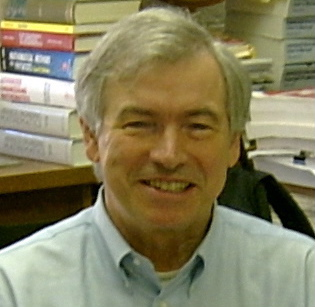
\includegraphics[height=\the\HauteurDesPhotos]{Rice}\\%
Cherepanov&Rice%
\end{tabular}}
\medskip
\ImageADroite{%
Par la suite, des méthodes expérimentales ont été élaborées pour permettre la mesure des
propriétés de rupture de critiques à partir d'échantillons à l'échelle du laboratoire pour
des matériaux dans lesquels la dimension des prélèvements est insuffisante pour garantir la
validité les hypothèses de la mécanique linéaire élastique de la rupture, et d'en déduire
une valeur critique de l'énergie de rupture~$J_{1c}$.\\[+1ex]
\indent
La quantité $J_{1c}$ définit le point à partir duquel se forme une zone plastique dans le matériau
au moment de la propagation et pour un mode de chargement.}

\medskip
L'intégrale $J$\index{Intégrale $J$} est équivalente au taux de restitution de l'énergie de déformation
d'une fissure dans un solide soumis à une charge constante.\index{Taux de restitution d'énergie $G$}
Cela est vrai, dans des conditions quasi-statiques, tant pour les matériaux linéairement élastiques que
pour les échantillons expérimentés à petite échelle en passe de céder en front de fissure.
\end{histoire}

Considérons un solide linéaire élastique homogène 2D sur lequel agissent des force $T_k$.
Les efforts de traction s'écrivent $T_i=\sigma_{ij}n_j$ (où $n$ est la normale sortante à $\Gamma$).
La densité d'énergie interne élastique est:
\begin{equation}
\omega=\dint_0^{\varepsilon_{kl}} \sigma_{ij}\dd\varepsilon_{ij}
\end{equation}
On travaille en l'absence de forces de volumes, d'où $\sigma_{ij,i}=0$, et sous hypothèse de petites déformations, soit $\varepsilon_{ij}=(u_{i,j}+u_{j,i})/2$.
\begin{figure}[ht]
\centering
\subfloat[titre ?]{\includegraphics[height=55mm]{j1.eps}}
\subfloat[titre ?]{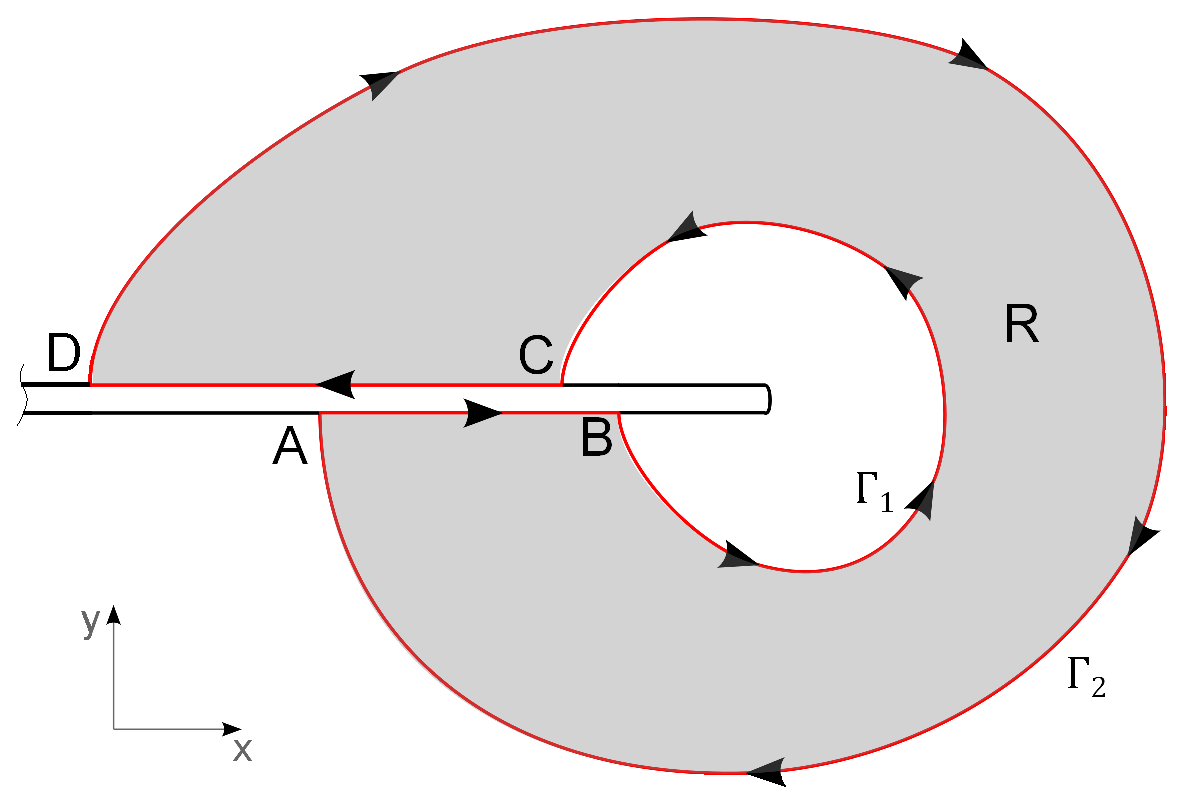
\includegraphics[height=55mm]{j3.eps}}
\caption{Titre ?}
\end{figure}
Les intégrales curvilignes:
\begin{equation}
Q_j =\dint_\Gamma \left(\omega n_j- T_k u_{k,j}\right)\dd\Gamma,\qquad j, k=1,2,3
\end{equation}
peuvent s'écrire:
\begin{equation}
Q_j =\dint_\Gamma \left(\omega n_j- \sigma_{lk}n_l u_{k,j}\right)\dd\Gamma
=\int_\Gamma \left(\omega \delta_{jl}- \sigma_{lk} u_{k,j}\right)n_l \dd\Gamma
\end{equation}
Le théorème de divergence puis quelques manipulations de l'opérande permettent d'arriver au résultat
suivant: \textcolorblue{$Q_j = 0$}. De là, on en tire que la densité dénergie interne élastique
\begin{equation}\omega=\dint_0^{\varepsilon_{kl}} \sigma_{ij}\dd\varepsilon_{ij}\end{equation}
est indépendante du chemin dans l'espace des déformations.
Le même type de calcul permet de montrer que la densité d'énergie complémentaire:
\begin{equation}\Omega = \dint_0^{\sigma_{kl}} \varepsilon_{ij}\dd\sigma_{ij}\end{equation}
est indépendante du chemin dans l'espace ds contraintes.

\medskip
On considère toujours notre solide linéaire élastique homogène 2D sur lequel agissent des
force~$T_k$. On définit \textcolorblue{l'intégrale $J$} comme:
\begin{equation} J = Q_1 =\dint_\Gamma \left(\omega n_1- T_k u_{k,1}\right)\dd\Gamma \end{equation}
D'après ce qui précède, \textcolorblue{$J=0$}, et donc
\begin{equation}J_1=\dint_{\Gamma_1} ... = J_2=\dint_{\Gamma_2} ...\end{equation}


Considérons maintenant une entaille (fissure) dans une pièce.
Alors, on a vu que l'intégrale $J$\index{Intégrale $J$} est nulle le long du chemin fermé $AB\Gamma_1CD\Gamma_2A$.
Si sur $AB$ et $CD$: $dy=0$, $T_k=0$, alors $J_{AB}=J_{CD}=0$
et il vient: $J_{\Gamma_1} = J_{\Gamma_2}$

\medskip
Rice\index[aut]{Rice (James R.), 1940-, Américain} a également démontré que la valeur de
l'intégrale $J$\index{Intégrale $J$} représente le taux de relaxation
d'énergie\index{Taux de restitution d'énergie $G$} pour la propagation des fissures planes,
ou le taux de diminution d'énergie potentielle par rapport à l'accroissement de la fissure, i.e. $J=G$.

\medskip
L'intégrale $J$ a été développée pour résoudre des difficultés rencontrées dans le calcul des
contraintes aux abords d'une fissure dans un matériau linéairement élastique.
Rice\index[aut]{Rice (James R.), 1940-, Américain} a montré qu'en mode de chargement constant et
sans atteindre l'adaptation plastique, l'intégrale $J$\index{Intégrale $J$} peut aussi être utilisée pour
calculer le taux de relaxation d'énergie dans un matériau plastique.\index{Taux de restitution d'énergie $G$}






\medskip
\section{Mécanique élastoplastique de la rupture}

Nous avons déjà mentionné que l'analyse linéaire élastique en mécanique de la rupture
ne s'applique que pour les matériaux fragiles.
En effet, dans la plupart des cas, il existe des déformations plastiques au fond de
fissure.

Si l'on suppose que cette zone plastique est présente dans un rayon $R$ autour
du fond de fissure, et qu'au delà, jusqu'à un rayon $D$ la solution singulière est
dominée par $K$; alors $R \ll D$ alors on peut considérer que la solution est dominée
par le facteur d'intensité de contrainte K.

Si $R$ n'est pas petit devant $D$, alors il faut tenir compte de la plastification locale.

\medskip
\subsection{Détermination de la zone plastique}

L'idée générale est de déterminer le lieu géométrique des points où le
champ de contraintes atteint la limite élastique du matériau.
\begin{figure}[ht]\centering
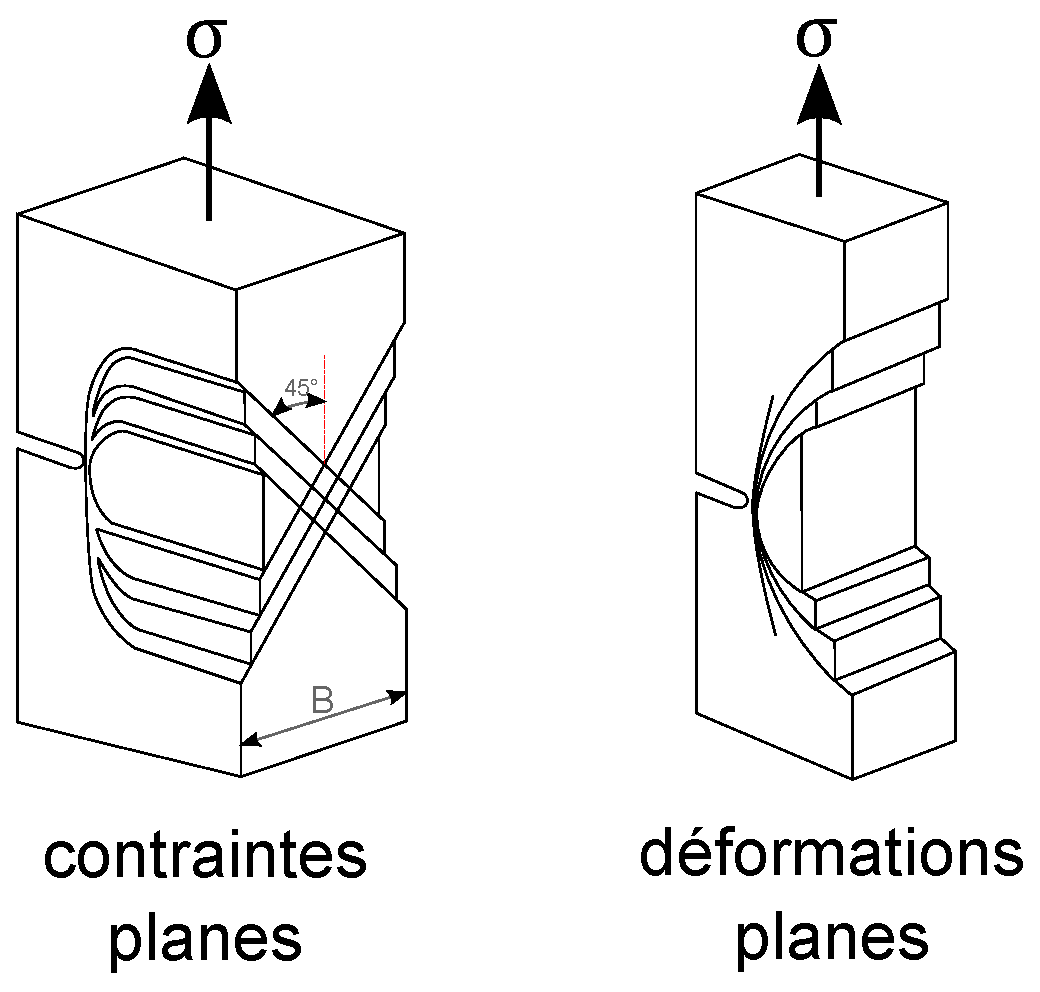
\includegraphics[height=50mm]{plast.eps}
\caption{Titre ?}\label{fig:propagation}
\end{figure}
Évidemment, en fonction du type de matériau, des hypothèses cinématiques...
cette zone peut être plus ou moins grande.

\medskip
Par exemple, pour un matériau isotrope et un critère de von Mises, la zone plastique en
contraintes planes est 9 fois plus grande que celle en déformations planes.

\medskip
Les chemins de propagation de la plasticité suivant l'épaisseur sont, dans ces deux cas,
illustrés sur la figure~\ref{fig:propagation}.


\medskip
\subsection{Modèle d'Irwin}
En 1960, Irwin\index[aut]{Irwin (George Rankine), 1907-1998, Américain} a présenté un modèle
de détermination de la zone plastique le long de l'axe  de la fissure sous l'hypothèse d'un matériau
élastique-plastique parfait, et en contraintes planes.

La zone plastique est donnée par:
\begin{equation}r_p(0)=\frac1{2\pi}\left(\frac{K_I}{\sigma_Y}\right)^2
\end{equation}$\sigma_Y$ étant la limite élastique.
Par conséquent, si $0<r<r_1$, $\sigma_2=\sigma_Y$ et lorsque $r>r_1$, $\sigma_2=\frac{K_I}{\sqrt{2\pi r}}$.
Comme $\sigma_2=\sigma_Y$ est constant pour $r < r_1$, il y a violation d'équilibre suivant l'axe $y$.
La réduction de $\sigma_2$ est compensée par $\sigma_1$ d'où une augmentation de $r_1$.
On obtient une zone plastique corrigée deux fois plus grande:
\begin{align}
&c = \frac1\pi\left(\frac{K_I}{\sigma_Y}\right)^2 \qquad \text{ en contraintes planes}\\
&c = \frac1{3\pi}\left(\frac{K_I}{\sigma_Y}\right)^2 \qquad \text{ en déformations planes}
\end{align}
et à l'extrémité de la fissure, l'ouverture est $\delta$:
\begin{align}
&\delta = \frac4{\pi E}\frac{K_I^2}{\sigma_Y} \qquad \text{ en contraintes planes}\\
&\delta = \frac{4(1-\nu^2)}{3\pi E}\frac{K_I^2}{\sigma_Y} \qquad \text{ en déformations planes}
\end{align}

\medskip
\subsection{Autres modèles}
\medskip
\subsubsection{Modèle de Dugdale}\index[aut]{Dugdale (Donald Stephen)}

Il s'agit d'un modèle valable pour les plaques très minces et constituées d'un matériau plastique
parfait avec critère de Tresca,\index[aut]{Tresca (Henri Édouard), 1814-1885, Français} et
où la plasticité est concentrée le long de l'axe de la fissure.

\medskip
\subsubsection{Critère de rupture basé sur l'ouverture de fissure}

Cette approche, introduite en 1961 par Wells\index[aut]{Wells (Alan Arthur), 1924-2005, Anglais} et
Cottrell,\index[aut]{Cottrell (Alan Howard, Sir -), 1919-2012, Anglais} postule qu'il y a initiation de fissures
en présence de plasticité, lorsque $\delta=\delta_c$.

On peut se servir du modèle d'Irwin\index[aut]{Irwin (George Rankine), 1907-1998, Américain} ou de celui de Dugdale (Burdekin et Stone)...


\medskip
\section{Modélisation numérique de la rupture}

\medskip
\subsection{Par la méthode des éléments finis}

Dans la formulation primale des éléments finis (dite formulation en déplacements), le
calcul fournit le champ de déplacement $u$ via les déplacements nodaux $\VV{q}$.
Le champ de déformations $\varepsilon$ est obtenu par dérivation des déplacements;
puis les contraintes sont obtenues via la loi de comportement:
\begin{equation}\sigma=H\varepsilon\end{equation}
Si le matériau est élastoplastique, les contraintes seront calculées de façon
incrémentale:
\begin{equation}\Delta\sigma=H(\sigma,\varepsilon)\Delta\varepsilon\end{equation}

\medskip
\subsubsection{Éléments finis singuliers}\index{Elément singulier}
Certains éléments ou configurations entraînent des \textcolorblue{singularités des déformations}.
Ce phénomène, que l'on cherche généralement soigneusement à éviter, est en fait idéal en
mécanique de la rupture.
Forcer les éléments à se comporter en $1/\sqrt{r}$ permet d'améliorer considérablement la solution
même avec maillage grossier.
Cette singularité peut être obtenue en utilisant des éléments quadratiques et en déplaçant
les nœuds des milieux de coté de $1/4$.

\medskip
Considérons l'élément de référence 2D carré quadratique à 8 nœuds (souvent appelé Q8).
Ses fonctions de forme $N_i$ sont:
\begin{equation} \begin{array}{ll}
N_i = &\left[ (1+\xi\xi_i)(1+\eta\eta_i)-(1-\xi^2)(1+\eta\eta_i)-(1-\eta^2)(1+\xi\xi_i)\right]
\dfrac{\xi_i^2\eta_i^2}4 \\
& +
(1-\xi^2)(1+\eta\eta_i)(1-\xi_i^2)\dfrac{\eta_i^2}2  +
(1-\eta^2)(1+\xi\xi_i)(1-\eta_i^2)\dfrac{\xi_i^2}4
\end{array}\end{equation}

Supposons maintenant que les nœuds 5 et 8 soient déplacés de 1/4 vers le nœud 1 (qui est l'origine
du repère).
Les fonctions de forme des nœuds 1, 2 et 5, obtenus pour $\eta=-1$ sont:
\begin{equation} N_1= -\frac12\xi(1-\xi) \quad
  N_2 = \frac12\xi(1+\xi) \quad
  N_5 = (1-\xi^2)
\end{equation}
et le calcul de $x(\xi,\eta)$ donne:
\begin{equation} x = -\frac12\xi(1-\xi)x_1 + \frac12\xi(1+\xi)x_2 + (1-\xi^2)x_5 \end{equation}
\begin{figure}[ht]\centering
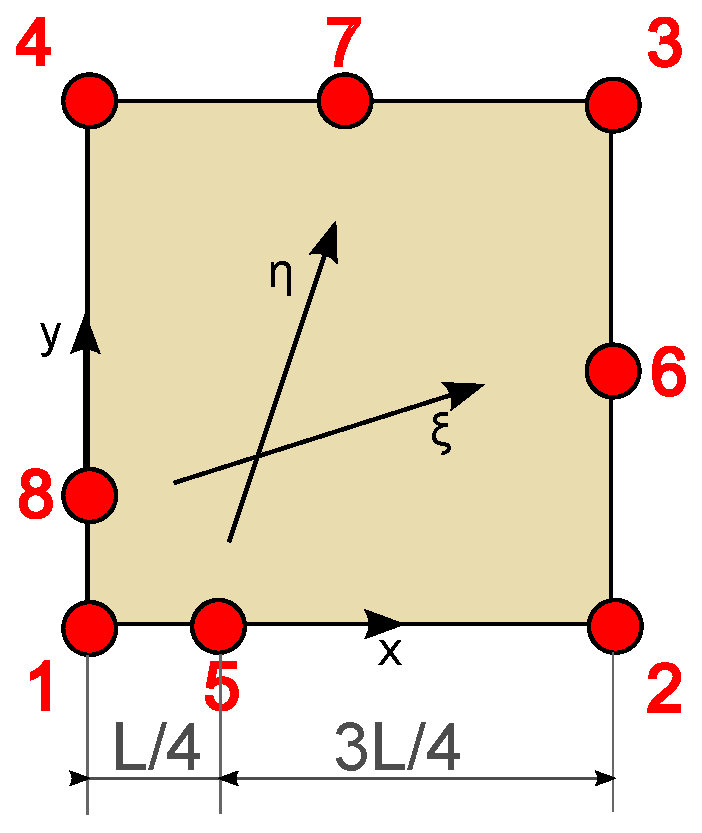
\includegraphics[height=45mm]{EltSing.eps}
\caption{Titre ?}
\end{figure}
soit pour $x_1=0$, $x_2=L$ et $x_5=L4$:
\begin{equation} x = \frac12\xi(1+\xi)L + (1-\xi^2)\frac{L}4 \quad \text{ et par suite: }
\xi=-1+2\sqrt{\frac{x}L} \end{equation}
Le terme du jacobien est $\frac{\partial x}{\partial\xi}=\frac{L}2(1+\xi)=\sqrt{xL}$
qui s'annule pour $x=0$ conduisant à une singularité des déformations.

Si l'on calcule  la déformation $\varepsilon_x$ le long du côté $1-2$, on trouve:
\begin{equation} \varepsilon_x = \dfrac{\partial u}{\partial x} =
-\frac12\left( \frac3{\sqrt{xL}}-\frac4L\right)u_1 + \frac12\left(-\frac1{\sqrt{xL}}+\frac4L\right)u_2
+\left(\frac2{\sqrt{xL}}-\frac4L\right)u_5 \end{equation}
qui est bien en $1/\sqrt{x}$.

\medskip
\subsubsection{Techniques numériques de calcul de $K$, $G$, $J$}

Il est possible d'effectuer un \textcolorblue{post-traitement des contraintes} en créant
un repère local centré sur la pointe de la fissure et en calculant la variable
$\sigma_{22}\sqrt{2\pi r}$ en chaque point de Gauss.\index[aut]{Gau\ss{} (Johann Carl Friedrich), 1777-1855, Allemand}

\medskip
On peut également \textcolorblue{post-traiter les déplacements} en les pondérant en fonction
de l'état de contrainte théorique censé s'appliquer sur la fissure.
%%%%%%%%%%%%%%%%%%%%
\medskipvm
Le taux d'énergie libérée de Griffith\index[aut]{Griffith (Alan Arnold), 1893-1963, Anglais} peut être
obtenu par la technique de \textcolorblue{progression de fissure} dans laquelle on effectue deux calculs EF:
l'un pour une fissure de dimension $a$, l'autre pour une fissure de dimension $a+\Delta a$.
En post-traitant l'énergie interne de toute la structure, on trouvera $G=-\Delta\Pi/\Delta a$.
\textcolorred{Si cette méthode est plus précise que les deux précédentes, elle nécessite deux
calculs EF.}

\medskip
Un \textcolorblue{calcul par dérivation de la rigidité} peut aussi être effectué.
Le but est encore une fois d'essayer de calculer $G=-\Delta\Pi/\Delta a$.
L'énergie potentielle étant donnée, dans le cas de l'élasticité linéaire, par:
\begin{equation}\Pi = \frac12\LL{q}\MM{K}\VV{q}-\LL{q}\VV{F}\end{equation}
Le calcul de $G$ conduit à:
\begin{equation}G = -\frac12\LL{q}\dfrac{\partial\MM{K}}{\partial a}\VV{q} =
-\frac12\LL{q}\left(\dsum_{i=1}^N \dfrac{\partial\MM{k_i}}{\partial a}\right)\VV{q}\end{equation}

\textcolorred{Cette méthode ne fait certes intervenir qu'un seul calcul EF, mais elle nécessite
un développement de code de dérivation des matrices de rigidité.}

\medskip
Si l'on a bien suivi, on a vu que \textcolorblue{l'intégrale $J$} est un outil bien adapté: ne
dépendant pas du contour, \textcolorred{cette intégrale n'est que peu sensible à la qualité du maillage}.
La plupart des codes actuels permettent de calculer cette intégrale $J$ sur un chemin
défini par l'utilisateur.



\medskip
\subsection{Par les méthodes sans maillage}\index{Méthode sans maillage}

La MEF souffre des limitations suivantes:
\begin{itemize}
   \item  La création de maillage pour des problèmes industriels est une tâche qui reste
	difficile et coûteuse;
   \item  En général les champs de contraintes EF sont discontinus, donc peu précis (mais
	nous avons vu comment y remédier...);
   \item  Distorsion des éléments en grandes déformations (ou alors régénération
	d'éléments, ce qui est une technique compliquée);
   \item  Difficulté de prédiction des chemins de propagation de fissures (ne passant pas par
	les nœuds), doublée de la difficulté de remailler automatiquement pour le suivi de
	propagation de fissures
   \item  Difficulté de représentation de l'effritement de matériau (impacts, explosifs,...).
\end{itemize}
Une idée <<~simple~>> est d'éliminer les éléments...

\medskip
Une brève description de la méthode est donnée au paragraphe \ref{Sec-meshless}.


\medskip
\subsection{Par les éléments étendus}\index{Méthode des éléments finis étendue}

La méthode des éléments finis étendus (X-FEM)\index{X-FEM} est rapidement présentée au
paragraphe \ref{Sec-XFEM}.

\medskip
Les éléments finis classiques ayant du mal avec les fortes discontinuités, on procède
à une enrichissement des éléments, dans les zones de discontinuités.

L'enrichissement peut être interne (ou intrinsèque) ou externe (ou extrinsèque).

Le principe consiste à augmenter la qualité de l'approximation des fonctions en ajoutant
à l'approximation déjà présente des informations sur la solution exacte (et donc sur
l'approximation du problème spécifique que l'on souhaite résoudre).







%VM OLD
\medskip
\section{Fatigue et durée de vie}

\medskip
\textcolorred{Dans ce paragraphe, nous nous placerons dans le cas des matériaux composites},
même si les démarches présentées sont pour beaucoup applicables à tous types
de matériaux.

\medskip
À l'heure actuelle, \textcolorblue{la question des critères de propagation en dynamique de la rupture
restent un sujet ouvert.}
Bien que de nombreux essais de propagation dynamique de fissure aient été effectués
ces dernières décennies, on se heurte à  l'absence de méthodes numériques suffisamment
fiables pour identifier les paramètres d'éventuels critères et comparer leur pertinence.
Par ailleurs, de tels essais sont difficiles à mettre en œuvre.

\medskip
Nous nous intéressons à des matériaux soumis à des sollicitations de faible intensité,
qui individuellement ne présenteraient pas de danger, mais qui appliquées de façon cyclique
conduisent à l'amorçage, puis à la propagation de fissures

Tant que les fissures restent suffisamment petites, il n'y à a pas de risque de rupture.
Le risque survient lorsque les microfissures (qui ne sont pas étudiées) grandissent (ou
se connectent) pour former des macrofissures auxquelles on peut appliquer ce qui a été dit avant.

\medskip
\subsection{Courbe et limite de fatigue}\index{Courbe de Wöhler (ou S-N)}

La courbe de Wöhler\index[aut]{Woehler@Wöhler (August), 1819-1914, Allemand}\index{Courbe de Wöhler (ou S-N)}
ou courbe S-N (pour Stress vs Number of cycles) de beaucoup de CFRP et
GFRP peut être décrite (entre $10^3$ et $10^6$ cycles) par une équation de la forme:
\begin{equation}    \dfrac{\sigma_a}{\sigma_u}=1-b\log N \end{equation}
où $\sigma_a$ et $\sigma_u$ sont la contrainte appliquée et la
résistance ultime, $N$ le nombre de cycle et $b$ une constante.

\medskip
La plupart des données disponibles en fatigue montrent une dispersion
élevée pour les courbes S-N. L'analyse statistique est alors inévitable.

\medskip
D'après Talreja, il existe une limite de déformation en fatigue
des composites, décrite comme la déformation minimale requise pour
initier un mécanisme d'endommagement de faible énergie.
Il suggère que pour les UD à base d'époxyde, cette limite est
autour de 0.6\%.


\medskip
\subsection{Cumul des dommages: principes de Miner}\index[aut]{Miner}

\medskip
Les essais de fatigue en laboratoire consistent généralement à répéter une même
sollicitation un grand nombre de fois. Dans ce cas, il est facile de définir un dommage : c'est
le nombre de répétitions de l'événement endommageant depuis le début de l'essai.

Dans le cas général, il y a plusieurs événements endommageants, qui diffèrent les uns
des autres par la grandeur des contraintes subies et par d'autres paramètres. Miner a proposé
deux principes qui permettent de cumuler les dommages:
\begin{itemize}
    \item Le dommage causé par une occurrence d'un événement est mesuré par l'inverse
	$1/N$ du nombre $N$ de fois qu'il faut répéter cet événement pour mener la pièce de
	l'état neuf jusqu'à la défaillance.
    \item Le dommage causé par une succession d'événements est la somme des dommages
	causés par chacun d'eux.
\end{itemize}

\medskip
Remarquons que ces deux principes sont cohérents. Si l'on suppose qu'un même événement
cause toujours le même dommage, et si l'on impose comme unité de dommage le dommage qui
conduit le système jusqu'à la défaillance, alors le premier principe est une conséquence du second.

Si $1 / N_A$ est le dommage de l'événement A et si $n_A$ est le nombre d'occurrences de cet
événement au cours d'un essai ou d'une utilisation du système alors le dommage total $D$
causé par tous les événements A, relativement à une défaillance, est défini par l'équation
de Miner:\index[aut]{Miner}
\begin{equation}  D = n_A / N_A  \end{equation}

\medskip
\textcolorblue{Avec cette définition, le dommage cumulé est égal à 1 au moment où la pièce se rompt.}

Il faut nuancer cette affirmation : des pièces apparemment identiques soumises aux mêmes
sollicitations se rompent en général au bout de nombres de cycles différents.
\textcolorred{La dispersion des durées de vie peut être très importante.}

 On trouve par expérience que les durées de vie
peuvent varier d'un facteur 5 ou 10 pour des pièces issues d'un même lot de production.
Il faut donc préciser davantage la formulation de la règle de Miner:\index[aut]{Miner}
s'il faut en moyenne $N_A$  répétitions de l'événement A pour qu'une défaillance survienne
alors le dommage causé par une occurrence de A est mesuré par $1 / N_A$.

\medskip
Les principes de Miner\index[aut]{Miner} permettent de définir le dommage causé par un événement
et affirment  que pour cumuler les dommages, il suffit de les additionner.

Ils imposent en outre le choix de l'unité
de dommage. Remarquons qu'il est toujours possible de changer d'unité. Par exemple, lorsqu'il y a
un seul événement endommageant, il est naturel de choisir comme unité de dommage le dommage
causé par une occurrence de cet événement.

\medskip
Les principes de Miner\index[aut]{Miner} permettent d'établir l'égalité des endommagements produits par des
événements de natures différentes. En particulier, ils permettent de préciser quand un petit nombre
d'événements de grande amplitude produit un endommagement égal à un grand nombre
d'événements de faible amplitude. Cela revêt une grande importance lorsqu'il faut définir
un essai aussi court que possible.



\medskip
\subsection{Propagation: loi de Paris}\index[aut]{Paris}\index{Loi de Paris}

\medskip
Pour une singularité caractérisée par sa dimension $a$ et sa forme, on étudie les courbes
$da/dN - \Delta K$ (où $N$ est le nombre de cycles et $\Delta K$ la variation du facteur
d'intensité de contrainte sur un cycle).

\medskip
\textcolorblue{Ces courbes, dont la partie centrale est linéaire, présentent deux asymptotes pour $da/dN$ et $\Delta K$
faibles et pour $da/dN$ et $\Delta K$ grands.}

la valeur mini vers laquelle tend la courbe est $\Delta K_S$, la valeur maxi $\Delta K_{Ic}$.
$K_{Ic}$ est la valeur critique qui correspond à une rupture instantanée par dépassement de la
valeur critique de $K$ sous chargement monotone.

$K_S$ est la valeur en dessous de laquelle il n'y à pas de propagation de fissure, c'est un
facteur d'intensité de contrainte seuil.

\medskip
\textcolorblue{Concernant la partie linéaire de ces courbes dans un diagramme log-log}, cela permet de les
modéliser par la loi de Paris (la plus simple des lois de propagation) qui définit la vitesse de
propagation par cycle comme une fonction puissance de l'amplitude du facteur d'intensité de
contrainte :
\begin{equation} \dfrac{da}{dN} = C.\Delta K^m \end{equation}
où $C$ et $m$ sont des coefficients dépendant du matériau.

La dimension critique de la singularité  $a_c$  est liée à la caractéristique du matériau $K_{IC}$,
la ténacité, elle entraîne la rupture  fragile de la structure :
\begin{equation} K_{IC} = F \sigma \sqrt{\pi a_c} \end{equation}
où $\sigma$ est une contrainte effective dans une direction normale à la fissure et $F$ un
facteur de forme.




\medskip
\subsection{Prédiction de la durée de vie}

Une fois un \textcolorred{indicateur d'endommagement choisi} (généralement la rigidité ou la
résistance résiduelle, la première pouvant être mesurée de manière non
destructive), on utilise :
\begin{itemize}
   \item \textcolorblue{\em théories empiriques:} les courbes S-N\index{Courbe de Wöhler (ou S-N)} sont utilisées
         pour caractériser le comportement en fatigue du composite.
         Un nombre important d'essais est nécessaire pour chaque
         configuration spécifique;

   \item \textcolorblue{\em théories de dégradation de résistance résiduelle:}
         elles sont basées sur l'hypothèse qu'un changement de la
         résistance résiduelle $\sigma_r$ en fonction du nombre de
         cycles $n$ est lié à la contrainte maximale appliquée $\sigma_a$.
         On a généralement une relation de la forme:
         \begin{equation}
            \dfrac{d \sigma_r}{d n} = -\dfrac1\gamma f\sigma_a^y
            \sigma_r^{1-\gamma}
         \end{equation}
         où $\gamma$ et $f$ sont des paramètres indépendants des
         contraintes mais qui peuvent dépendre de la température, de
         l'humidité, de la fréquence.
         Souvent, on suppose une distribution\index{Loi de Weibull}\index[aut]{Weibull (Ernst Hjalmar Waloddi), 1887-1979, Suédois}
        de Weibull
\footnote{En théorie des probabilités, la loi de Weibull,\index{Loi de Weibull}\index[aut]{Weibull (Ernst Hjalmar Waloddi), 1887-1979, Suédois} est une loi de probabilité continue. Avec deux paramètres sa densité de probabilité est :
\begin{equation*}   f(x;k,\lambda) = (k/\lambda) (x/\lambda)^{(k-1)} e^{-(x/\lambda)^k}\end{equation*}
où $k > 0$ est le paramètre de forme et $\lambda > 0$ le paramètre
d'échelle de la distribution.
Sa fonction de répartition est définie par
$   F(x;k,\lambda) = 1- e^{-(x/\lambda)^k}$,
où, ici encore, $x > 0$.
%%%%%%%%%%%%%%%%%%%%%%
\medskipvm
Une version généralisée  à trois paramètres existe.

\medskip
La distribution de Weibull est souvent utilisée dans le domaine de l'analyse de la durée de vie,
grâce à sa flexibilité, car elle permet de représenter au moins approximativement une
infinité de lois de probabilité.
Si le taux de panne diminue au cours du temps alors, $k < 1$.
 Si le taux de panne est constant dans le temps alors, $k = 1$.
Si le taux de panne augmente avec le temps alors, $k > 1$.
La compréhension du taux de panne peut fournir une indication au sujet de la cause des pannes:
\begin{itemize}
	\item un taux de panne décroissant relève d'une <<~mortalité infantile~>>. Ainsi, les
		éléments défectueux tombent en panne rapidement, et le taux de panne diminue
		au cours du temps, quand les éléments fragiles sortent de la population;
	\item un taux de panne constant suggère que les pannes sont liées à une cause stationnaire;
	\item un taux de panne croissant suggère une <<~usure ou un problème de fiabilité~>> :
		les éléments ont de plus en plus de chances de tomber en panne quand le temps passe.
\end{itemize}
On dit que la courbe de taux de panne est en forme de baignoire. Selon l'appareil, baignoire sabot ou piscine.
Les fabricants et distributeurs ont tout intérêt à bien maîtriser ces informations par type de produits
afin d'adapter :
   1. les durées de garantie (gratuites ou payantes)
   2. le planning d'entretien}%
de la résistance des composites. La rupture par fatigue survient lorsque la résistance résiduelle du composite est atteinte par la contrainte appliquée.

   \item \textcolorblue{\em théories de perte de rigidité:} ce sont des généralisations
         du cas précédent.

         Les plis les plus désorientés par rapport au chargement
         (éléments sous-critiques) commencent à s'endommager (ce
         qui est caractérisé par une perte de rigidité), ce qui cause
         une redistribution des contraintes au niveau local.
         La résistance des éléments critiques (les plis orientés
         dans le sens de la charge) est gouvernée par les équations
         de dégradation de résistance.
         Ces deux phénomènes (perte de rigidité des éléments
         sous-critiques et perte de résistance des éléments critiques)
         contribuent à la définition de la résistance résiduelle
         et donc à la durée de vie.

   \item \textcolorblue{\em théories d'endommagement cumulatif:} elle sont basées
         sur une observation expérimentale soigneuse et sur une
         simulation de l'accumulation de l'endommagement du
         sous-lamina.
         Il manque toutefois un critère de rupture des laminés sous
         chargement de fatigue tension-tension pour ces théories.
   \item \textcolorblue{\em théories d'endommagement continu:} l'endommagement
         est pris en compte par un paramètre $D$ sous la forme:
         \begin{equation}
            \widehat{\sigma}=\dfrac{\sigma}{1-D}
         \end{equation}
         où $\sigma$ et $\widehat{\sigma}$ sont la contrainte
         imposée et la contrainte effective après endommagement.
         L'avantage de cette approche est d'éviter la prise en
         compte de l'endommagement microstructural parfois difficile
         à modéliser et mesurer.
\end{itemize}


\medskip
Notons également que \textcolorred{pour obtenir les informations nécessaires, de nombreux essais doivent être
menés}, surtout parce que de nombreux facteurs conditionnement la fatigue des FRP:
\begin{itemize}
	\item \textcolorblue{fréquence}: un échauffement du matériau avec la fréquence de sollicitation est
		constaté. Il faudrait modifier ses lois de comportement.
	\item \textcolorblue{amplitude}: une sollicitation de grande amplitude suivie d'une sollicitation de faible amplitude
		conduit à une durée de vie inférieure au cas où l'ordre des sollicitations est
		inversé.
	\item \textcolorblue{$R=-1$} (rapport entre charge positive et négative dans le cyclage) : ce cas est très
		défavorable dans notre exemple car la tenue en compression est moins bonne qu'en
		traction (flambage des fibres et splitting...);
	\item \textcolorblue{la forme du signal} a une influence qui serait à considérer.
	\item \textcolorblue{séquence d'empilement}: les composites sont censés être conçus pour soutenir la
		charge dans le sens des fibres. Dans le cas de sollicitations complexes, les plis les
		moins bien orientés par rapport à la charge cèdent en premier...
	\item \textcolorblue{humidité};
	\item \textcolorblue{vieillissement naturel}...
	\item ...
\end{itemize}
\textcolorred{C'est un problème de structure car il y a couplage entre les modes d'endommagement à différentes échelles.}

\medskip
Dans ces cas simples, on peut utiliser un critère cumulatif de Miner ou des lois d'équivalence (par
exemple entre temps, fréquence, température...)



\medskip
\subsection{Sur la fatigue des composites}

Les remarques suivantes peuvent être faites, quant à la poursuite de
travaux de recherche sur le sujet:
\begin{itemize}
   \item Bien que la conception orientée par la rigidité pour les GFRP
         soit peu concernée par la contrainte de rupture, le fluage
         est un aspect fondamental de leur conception.
   \item Les effets de synergie entre le fluage et les autres types
         de chargement est un domaine à explorer.
   \item Peu de données de fatigue sont disponibles pour le domaine
         $10^7-10^8$ cycles (Les japonais ont des essais en cours).
   \item L'effet d'échelle sur les performance n'est pas clair.
         En particulier, il n'est toujours pas sûr qu'un tel effet
         existe.
   \item La représentativité des éprouvettes ou des tests accélérés
         restent des problèmes épineux.
   \item Les composites hybrides doivent être étudiés.
   \item La dégradation des GFRP à haute température n'est pas
         bien comprise.

         Toutefois, Tsotsis\index[aut]{Tsotsis (Thomas K.), ?- , Américain} et
	 Lee\index[aut]{Lee (Shaw M.), ?- , Américain} notent que le
         comportement à long terme des composites soumis à des
         températures élevées
         est contrôlé par les dégradations d'oxydation et thermique.
         Dans leur article, deux résines particulières sont étudiées.

   \item Les {\em composites épais ne sont pas étudiés}, tout comme
         l'influence de l'épaisseur.
         Pourtant, des mécanismes de ruptures suivant l'épaisseurs peuvent
         sans doute apparaître de manières différentes de celles des
         laminés plus fins: effet de taille ou interaction de mécanismes.
\end{itemize}
